	\subsection{Taxonomy of virtualization by \textit{Bugnion}}
	
	\begin{figure}[H]
		\centering
		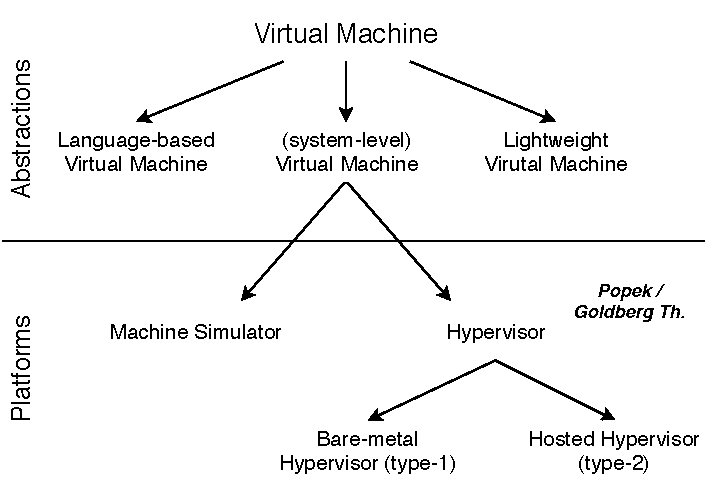
\includegraphics[width=8.5cm]{images/Bugnion2017.pdf}
		\vspace{-0.2cm}
		\caption{Basic classification of virtual machines and the platforms that run them by \textit{Edouard Bugnion, Jason Nieh, Dan Tsafrir and Margaret Martonosi} in 2017 \cite{Bugnion2017}.}
		\label{fig:TaxonomyOfVirtualizationBugnion}
	\end{figure}
	
    From the perspective of the work of Ameen and Asmaa \cite{Ameen2013}, there are many different types of virtualization. In its first level is located some domains as  Mobile, Data, Memory, Desktop, Storage, Server, Network, Application, Grid and Clustering. The second level shows the types considered for the Server Virtualization as Emulation, Hosted OS, Hardware, Paravirtualization, Container and Hybrid. Finally, the third level shows the types of virtualization considered for Hardware as Type 1 and Type 2. See figure \ref{fig:TaxonomyOfVirtualizationByAmeen}.
  
